%% Based on a TeXnicCenter-Template by Gyorgy SZEIDL.
%%%%%%%%%%%%%%%%%%%%%%%%%%%%%%%%%%%%%%%%%%%%%%%%%%%%%%%%%%%%%

%------------------------------------------------------------
%
\documentclass{article}%
%Options -- Point size:  10pt (default), 11pt, 12pt
%        -- Paper size:  letterpaper (default), a4paper, a5paper, b5paper
%                        legalpaper, executivepaper
%        -- Orientation  (portrait is the default)
%                        landscape
%        -- Print size:  oneside (default), twoside
%        -- Quality      final(default), draft
%        -- Title page   notitlepage, titlepage(default)
%        -- Columns      onecolumn(default), twocolumn
%        -- Equation numbering (equation numbers on the right is the default)
%                        leqno
%        -- Displayed equations (centered is the default)
%                        fleqn (equations start at the same distance from the right side)
%        -- Open bibliography style (closed is the default)
%                        openbib
% For instance the command
%           \documentclass[a4paper,12pt,leqno]{article}
% ensures that the paper size is a4, the fonts are typeset at the size 12p
% and the equation numbers are on the left side
%
\usepackage{amsmath}%
\usepackage{amsfonts}%
\usepackage{amssymb}%
\usepackage{graphicx}
%-------------------------------------------
\newtheorem{theorem}{Theorem}
\newtheorem{acknowledgement}[theorem]{Acknowledgement}
\newtheorem{algorithm}[theorem]{Algorithm}
\newtheorem{axiom}[theorem]{Axiom}
\newtheorem{case}[theorem]{Case}
\newtheorem{claim}[theorem]{Claim}
\newtheorem{conclusion}[theorem]{Conclusion}
\newtheorem{condition}[theorem]{Condition}
\newtheorem{conjecture}[theorem]{Conjecture}
\newtheorem{corollary}[theorem]{Corollary}
\newtheorem{criterion}[theorem]{Criterion}
\newtheorem{definition}[theorem]{Definition}
\newtheorem{example}[theorem]{Example}
\newtheorem{exercise}[theorem]{Exercise}
\newtheorem{lemma}[theorem]{Lemma}
\newtheorem{notation}[theorem]{Notation}
\newtheorem{problem}[theorem]{Problem}
\newtheorem{proposition}[theorem]{Proposition}
\newtheorem{remark}[theorem]{Remark}
\newtheorem{solution}[theorem]{Solution}
\newtheorem{summary}[theorem]{Summary}
\newenvironment{proof}[1][Proof]{\textbf{#1.} }{\ \rule{0.5em}{0.5em}}

\begin{document}

\title{Exploring and Modeling with the IMDB Movie Dataset}
\author{
\\University of Memphis}
\date{December 06, 2016}
\maketitle

\begin{figure}
\centering
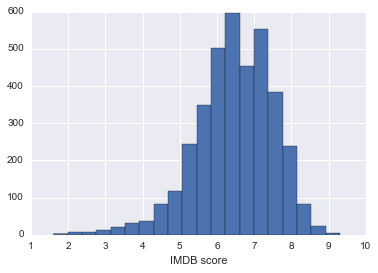
\includegraphics[width=1.0\columnwidth]{Fig/imdbhist.png}
\caption{Histogram plot for imdbscore}
\label{fig:imdbhist}
\end{figure}

\begin{figure}
\centering
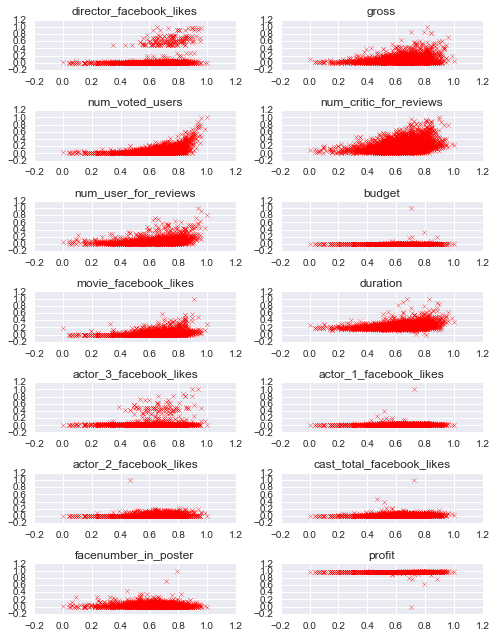
\includegraphics[width=1.0\columnwidth]{Fig/ScatterPlot.png}
\caption{Scatter plot for imdbscore v numerical features}
\label{fig:scatter}
\end{figure}

\begin{figure}
\centering
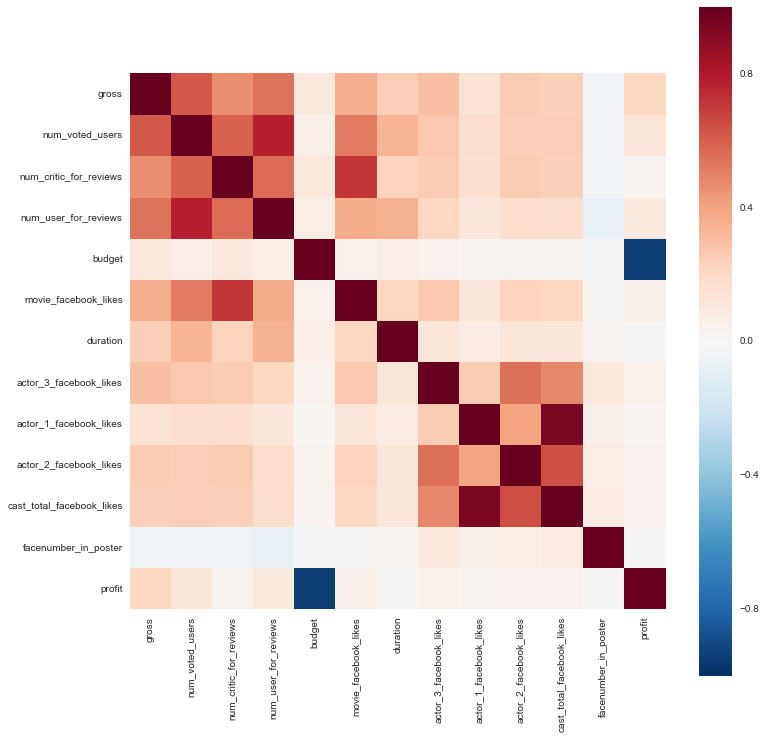
\includegraphics[width=1.0\columnwidth]{Fig/Correlationoffeatures.png}
\caption{Correlation of Numerical features}
\label{fig:Correlationoffeatures}
\end{figure}


\section{Introduction}

Movies can be of different stories, genre, from different countries, having different actors (both male and female), directors and others. There are several sources in the internet today that stream our favorite movies on demand, that is whenever you want and as often you want, Netflix for example. We all love to watch movies. It is one of the best entertainer during the leisure hours. 

\subsection{Goal Description}

We are interested to predict whether a movie is going to be popular or not or what will the gross income of a particular movie before its release or what will be the IMDB score of a movie or to suggest you a movie quite similar to the one who have just watched. This seems to be exciting, since based on our relied prediction one (from the audience) can go and watch a movie (predicted to be popular and entertaining) or based on the prediction of the gross, the movie makers can change their marketing regime for a particular movie,  before its release. 
In this work, we have done an exploratory analysis and modeling with IMDB movie data set available in an online data science platform, Kaggle. Namely, we have performed visualization, 'value' prediction or regression in the form of predicting the imdb score and gross of a movie, 'class' prediction or classification in the form of predicting the popularity of a movie, and clustering in the form of a basic recommender system.

\subsection{DataSet Description}

We used the IMDB 5000+ movie dataset for our project. The dataset consists of 5043 unique movies and their attributes (28 variables). The collection spans over 100 years and 66 different countries. There are 2399 unique director names and thousands of actors and actresses. The following is the list of 28 variables from the data set,

[movietitle, color, numcriticforreviews, moviefacebooklikes, duration, directorname, directorfacebooklikes, actor3name, actor3facebooklikes, actor2name, actor2facebooklikes, actor1name, actor1facebooklikes, gross, genres, numvotedusers, casttotalfacebooklikes, facenumberinposter, plotkeywords, movieimdblink, numuserforreviews, language, country, contentrating, budget titleyear, imdbscore, aspectratio.]

\section{Methodologies}
\subsection{Regression or 'Value' Prediction}
In this work we have developed regression models for predicting, \textit{imdbscore} and \textit{gross} of a movie. First we describe the analysis and methods used for \textit{imdbscore} prediction. \textit{imdbscore} is a score or rating provided to movies by critics by an online databased platform for movies, IMDB\cite{}. This score is able to quantify how popular a movie is. Figure~\ref{fig:imdb_hist} shows a histogram plot for the imdb scores. From the plot we can observe a normal distribution of the score, with a mean = 6.465$\pm$1.056, minimum value of 1.6 for the movie \textit{Justin Beiber: Never say never} and maximum of 9.3 for the movie \textit{Shawshank Redemption}. 
In the data set, we have 28 variables, out of which there are 13 useable numeric features, namely, [directorfacebooklikes, gross, numvotedusers, numcriticforreviews, numuserforreviews, budget, moviefacebooklikes, duration, actor3facebooklikes, actor1facebooklikes, actor2facebooklikes, casttotalfacebooklikes, facenumberinposter], and we have included the profit of a movie, which is calculated by subtracting the budget from the gross. First, we have cleaned the data by dropping those samples having NaN values (using 3756 out of 5043 for modeling) and scaled all the features. For all analysis we have used the numpy, scipy, sklearn, pandas, matplotlib, seaborn and bokeh libraries of python.

\subsection{Prediction of ImdbScore}
\begin{itemize}
\item Initial step: Since this is a regression problem, we just run a simple linear regression using all the numerical features. To be noted for all the linear regression models, we have performed evaluation by running different folds of the training and test samples, that is with trainsize = 0.5, 0.66 and 0.75 and report the mean residue square value and the mean square error. We observe the following results. The mean MSE is 0.013 and mean residual square is $0.296$.
\end{itemize}

\begin{itemize}
\item Second step: Next we analyzed the correlation of these features with the \textit{imdbscore} as shown via the scatter plots in figure~\ref{fig:scatter}. We observe that \textit{numvotedusers} has the highest correlation with \textit{imdbscore}, 0.482 and \textit{facenumberinposter} has a negative correlation of -0.065. We observe that for \textit{directorfacebooklikes} (642 out of 3756 are 0) and \textit{moviefacebooklikes} (1742 out of 3756 are 0) has a lot of missing data, hence, we remove them from our next analysis. Next we again performed a simple linear regression for predicting the \textit{imdbscore}, with the new set of features. We observe the following results. The mean MSE is 0.0126 and mean residual square is 0.323. We observe an improvement from the first step.
\end{itemize}

\begin{itemize}
\item Third step: Next we observe that there are a few text features that might be useful in predicting the \textit{imdbscore}, namely \textit{genre}, \textit{plotkeywords} and \textit{country}, we need to add these to the numerical features. For this, first we obtain the tfidf scores with the tfidf vectorizer and use todense() to convert each feature from sparse to dense matrix. Next we append these feature along with the numerical features to obtain a new feature list to predict the \textit{imdbscore}. We observe the following results. The mean MSE is 0.011 and mean residual square is 0.455. We observe an improvement from the second step.
\end{itemize}

\begin{itemize}
\item Fourth step: Next from the figure~\ref{fig:Correlationoffeatures}, we observe that some of the features are correlated to each other. For example, \textit{numvotedusers} and \textit{numcriticforreviews} have some correlation, similarly \textit{gross} and \textit{numvotedusers} have some correlation, hence in this step we have used LASSO regression, since this method does feature selection by assigning 0 coefficient for those features which are redundant and hence reduces overfitting via first norm regularization. We use aic/bic for evaluating the model. We have found the optimal alpha from a range of alpha values of the LASSO model for which the aic and bic are minimum. We performed cross validation to obtain a mean cross-validation score of 0.471. We observe an improvement from the third step.
\end{itemize}

\begin{itemize}
\item Fourth step: Next from the figure~\ref{fig:Correlationoffeatures}, we observe that some of the features are correlated to each other. For example, \textit{numvotedusers} and \textit{numcriticforreviews} have some correlation, similarly \textit{gross} and \textit{numvotedusers} have some correlation, hence in this step we have used LASSO regression, since this method does feature selection by assigning 0 coefficient for those features which are redundant and hence reduces overfitting via first norm regularization. We use aic/bic for evaluating the model. We have found the optimal alpha from a range of alpha values of the LASSO model for which the aic and bic are minimum. We performed cross validation to obtain a mean cross-validation score of 0.471. We observe an improvement from the third step.
\end{itemize}

\begin{itemize}
\item Fifth step: Next we attempted using the Random Forest Resgression to perform the prediction of the \textit{imdbscore}. We performed 5-fold cross validation for the evaluation. We observed the mean cvScore to be 0.511. Another important aspect of random forest is that it provides us with the feature importance list. We note the following top 10 features for \textit{imdbscore} prediction. [numvotedusers, genres, budget, duration, numuserforreviews, gross, numcriticforreviews, directorfacebooklikes, actor3facebooklikes, profit]. 
\end{itemize}

\begin{figure}
\centering
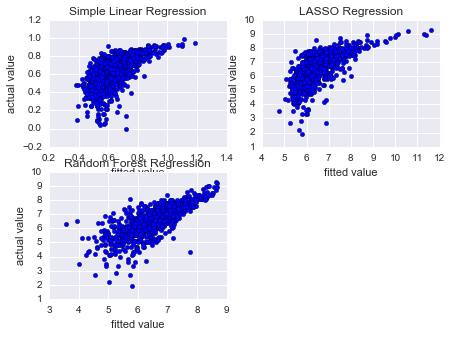
\includegraphics[width=1.0\columnwidth]{Fig/Fitplot.png}
\caption{Fitted vs Actual data plot}
\label{fig:Fitplot}
\end{figure}

Hence we conclude that random forest regression works best among all the methods used to predict the value of \textit{imdbscore} given the features of a movie. Figure~\ref{fig:Fitplot} shows the fitted vs actual data plot for the three methods used. 

\subsection{Prediction of Gross}



\end{document}
